%!TEX ROOT = thesis.tex
\chapter{Requirement}
\section{Hardware Requirement Introduction}
In this project, a smartphone is required. The smartphone must have Global Positioning System (GPS) and Bluetooth device. A OBD-II to Bluetooth adapter, ELM327 is required to use in data collection. The model of vehicle used to collect driver data should be year 2006 onward. Some of the brand can not be supported by the ELM327 due to the protocols mismatch. The ELM327 supports most of the vehicle model with year 2008 in Proton brand, Toyota brand, and Honda brand. However, the latest model of the vehicle may not be supported due to the protocols mismatch problem also.

\subsection{Vehicle OBD system}
The OBD system is also called OBD-II, was proposed in 1996. In 1996, all the cars manufactured in United State (US) were required to equip OBD-II and the cars without OBD-II prohibited to sell in US. The purpose to have OBD-II specifications is to diagnose engine problem. The specifications were being used by the Environment Protection Agency (EPA) and the state of California to meet the emission standards. Since 1996, all the cars in US are required to be equipped with OBD-II to establish the EPA regulation. 

The usage of the OBD-II is important for detecting the vehicle exhaustion. If the vehicle is exhaust high level of air-pollution content, Diagnostic Trouble Codes (DTCs) will be generated by the OBD-II and a Check Engine Light will be displayed on vehicle dashboard. OBD-II will store this DTCs into the  Engine Control Unit memory. An OBD-II scanning tool can access the ECU to retrieve the DTCs.

The OBD-II is usually installed under the vehicle dashboard and above the pedals. Figure \ref{fig:obd} shows the OBD-II socket of Toyota Vios year 2007 model.

\begin{figure}[hbt!]\centering
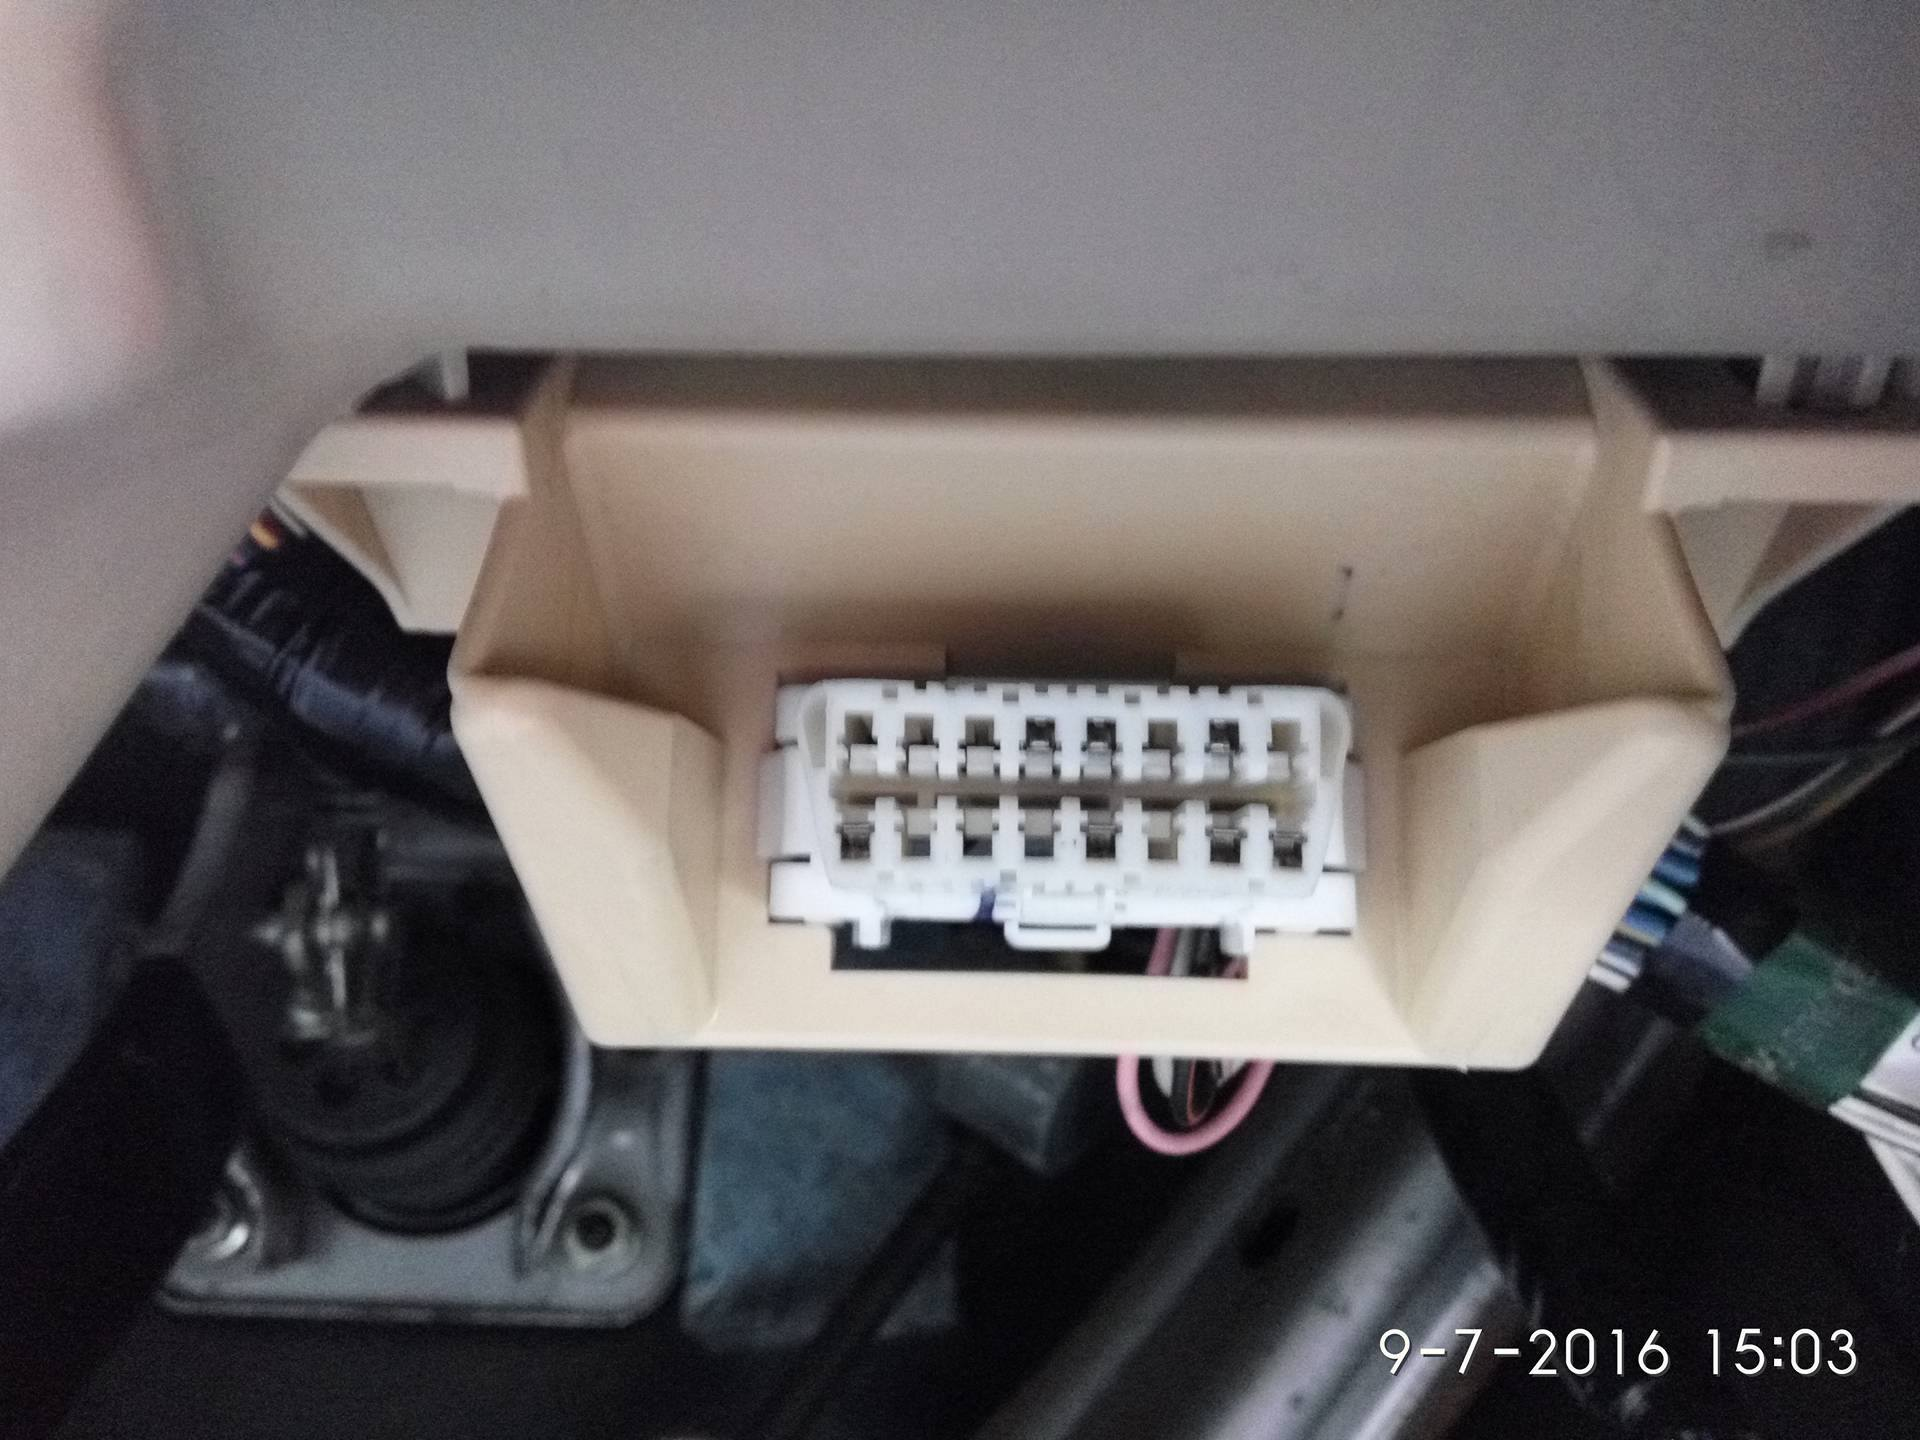
\includegraphics[width=.75\textwidth]{image/obd}
\caption{OBD-II socket of the Toyota Vios year 2007 model.}
\label{fig:obd}
\end{figure}

\subsection{ELM327}
Super Mini ELM327 Bluetooth OBD-II is an OBD-II scanning tool produced by ELM Electronics. It is a programmed micro-controller to communicate with the OBD-II port of the vehicle. The ELM327 supports most of OBD-II protocols. ELM327 also contains the Bluetooth adapter. The ELM327 needs to be plugged to the OBD-II port.

\begin{figure}[hbt!]\centering
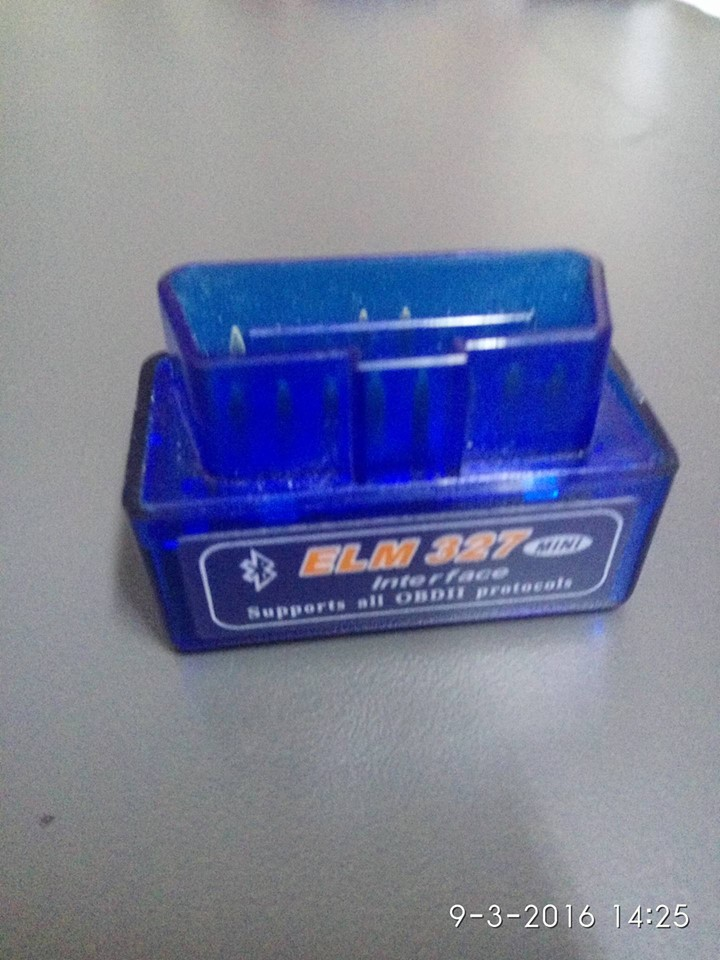
\includegraphics[height=.5\textheight]{image/ELM327}
\caption{Super Mini ELM327 Bluetooth OBD-II.}
\end{figure}

\section{Software Requirement Introduction}
In order to collect the vehicle operation data, Torque(Lite), an Android application needs to be installed in the smartphone. Vehicle operation data will be stored in smartphone with Comma Separated Values (CSV) file format. Google Drive will be utilized to store the CSV file as a cloud storage.

In order to add on the new features to the dataset, Google Sheet and LibreOffice are used for modifying the dataset. 

Google Earth are used for verify the road structure that drivers drove through. The Torque(Lite) can convert the CSV file to Keyhole Markup Language (KML) file.
 
LibreOffice are applied in this project to do the final modification of the data set. After the modification, the data set will be stored as CSV format file. KNIME Analytic Platform is used for clustering the collected vehicle operation data by performing K Means Algorithm. The result will be visualized by using Tableau.

\subsection{Torque(Lite)}
Torque Lite version is a free android application and it is able to be installed in smartphone from Google Play Store. The application will communicate with the ELM327 through the Bluetooth connection. The application will collect the data received from the ELM327 and  save the data into a CSV file in the smartphone. 

After vehicle ignition is on, ELM327 need to connect with the smartphone that operating Torque via Bluetooth. Once the smartphone connected with the adapter, Torque will choose the protocol that matches with the OBD-II system. After the matching successes, Torque will start to read the sensor information from the ECU. In order to collect the GPS data, smartphone's location service is required to be enabled at the same time. When the smartphone received GPS signal and connected with the adapter, there are four flashing icons at the top right of the main screen will stay solid with blue color. Figure \ref{fig:torque} shows a screen-shot of the Torque(Lite).

\begin{figure}[hbt!]\centering
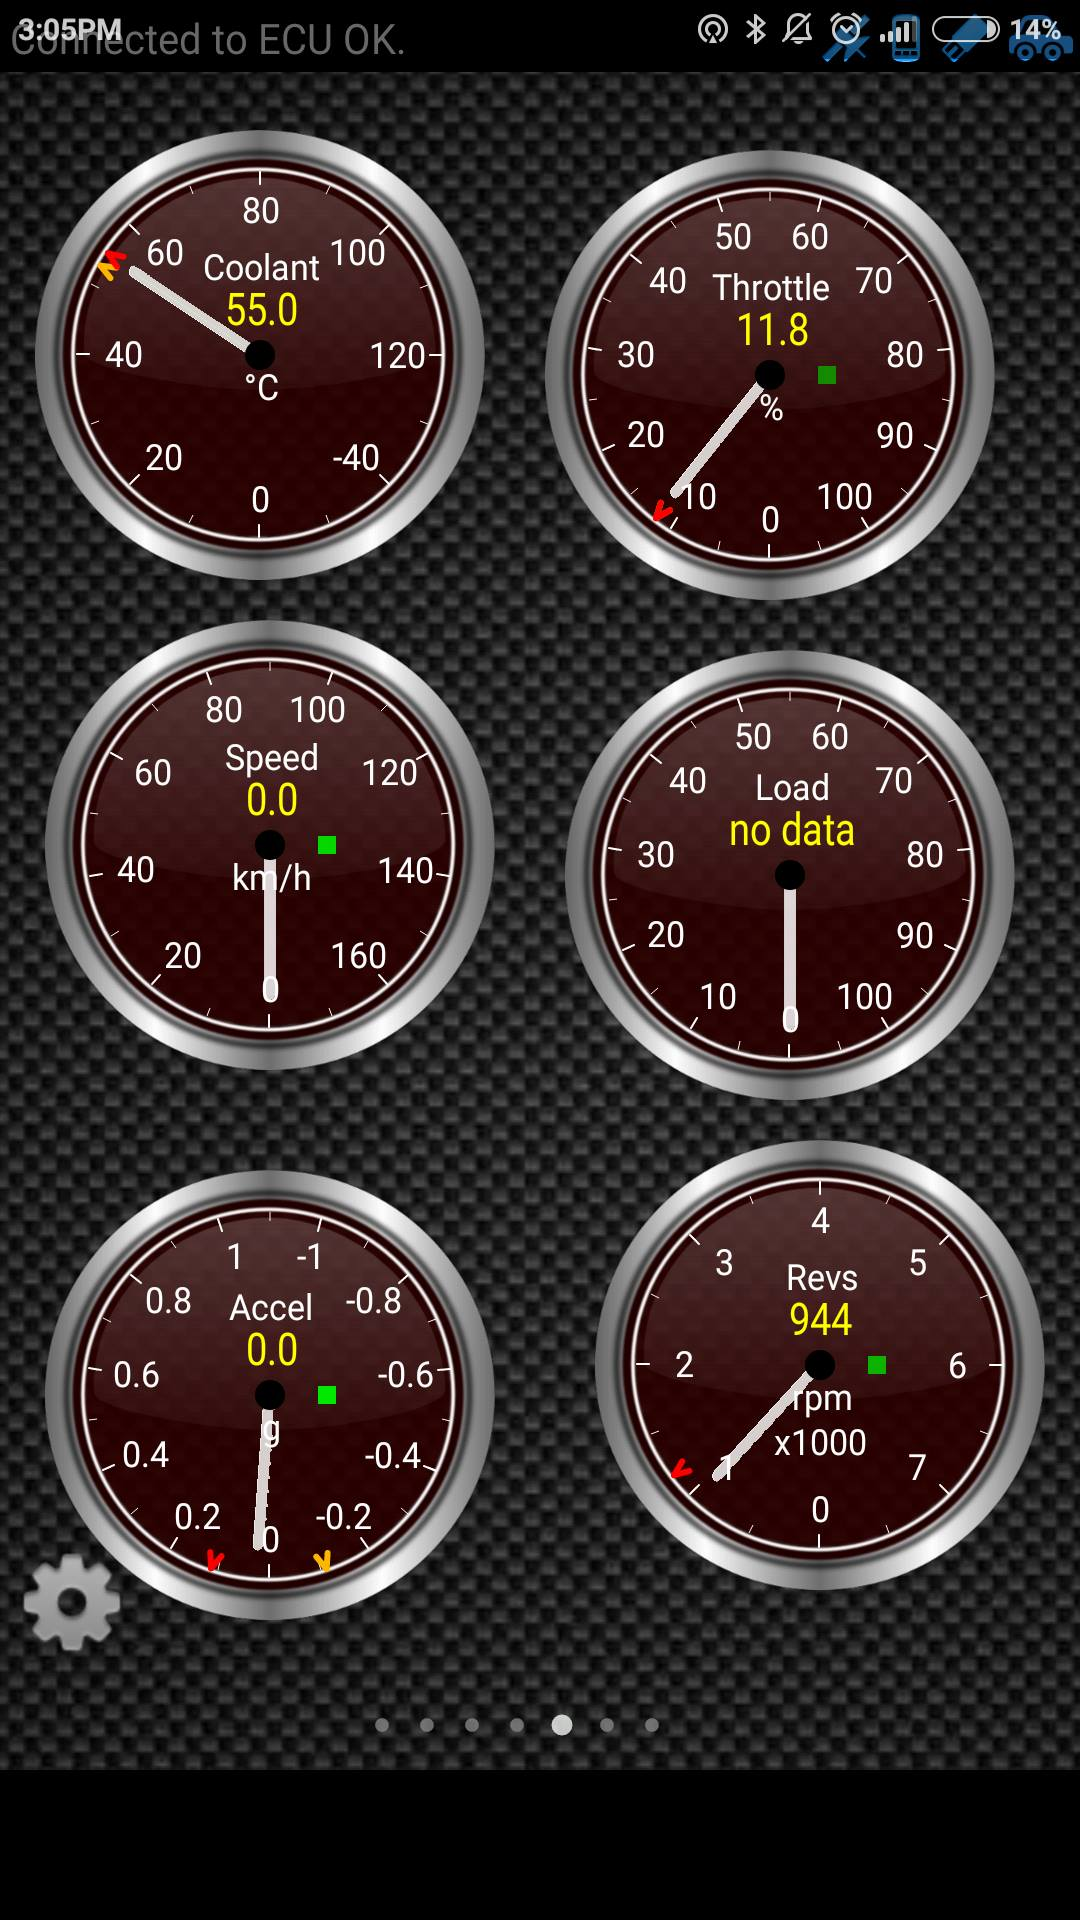
\includegraphics[height=.5\textheight]{image/torque}
\caption{Screen-shot of the Torque(Lite).}
\label{fig:torque}
\end{figure}

\subsection{KNIME Analytic Platform}
KNIME Analytic Platform is an open platform for data analysis. It is a perfect tool for data scientists. The version of KNIME Analytic Platform used in this project is version 3.2.0. 

KNIME Analytic Platform contain 1000 modules ,hundreds of ready-to-run examples, a set of integrated tools, and a list of advance algorithms available. User can build a machine learning experiment by dragging and dropping the related modules into the project. User needs to link and configure the module before execution.

This project uses the module of the KNIME Analytic to complete the data preprocessing and driving behavior modeling. K Means algorithm module is used in this project to classify the driving behavior.

\subsection{K Means Algorithm}
K Means algorithm is a popular clustering algorithm. The algorithm is used for automatically grouping data into cohesive 'clusters'. Few points will be initialized by choosing the training examples randomly. The number of the points is determined by the number of clusters wanted to be generated. For example, in order to get three clusters as output, three points is required to be initialized in the first step. The points are called cluster centroids \cite{andrew:2016}.

The second step of the algorithm is an inner loop for performing two functions. The functions are shown below:
\begin{enumerate}
\item Assign each training example to the closest cluster centroids.
\item Move the cluster centroids to the mean of the points assigned to it.
\end{enumerate} 

This looping will be ended when the new iterations do not make the cluster centroids moved.

\subsection{Tableau}
Tableau is an software that has powerful data visualization functions. The data can be expressed by using graphics or diagrams in an interactive way. The version of the Tableau used in this project is version 10.0.